\documentclass[a4paper, 10pt]{article}

\usepackage[french]{babel}
\usepackage[utf8]{inputenc}
\usepackage[T1]{fontenc}
\usepackage[top=3cm, bottom=3cm, left=3cm, right=3cm]{geometry}
\usepackage{lmodern, amsmath, amssymb, mathrsfs, graphicx, listings, tabularx, color, pgfplots, pgfplotstable, booktabs, titling, authblk, parskip, pgfplots, csquotes}
\usepackage{hyperref}
\usepackage[backend=biber, url=false, isbn=false, sorting=none, natbib]{biblatex}
\usepackage[labelfont=sc]{caption}
\usepackage[bottom]{footmisc}
\setlength\parindent{1cm}
\MakeOuterQuote{"}
\hypersetup{colorlinks, linkcolor=black, urlcolor=black}
\pgfplotsset{compat=1.15}
\addbibresource{biblio.bib}
\bibliography{biblio}
\newcommand{\HRule}{\rule{\linewidth}{0.5mm}}
\newcolumntype{Y}{>{\centering\arraybackslash}X}
\newcommand{\Var}{\mathrm{Var}}
\DeclareMathOperator*{\argmax}{arg\,max}

\begin{document}

\begin{titlepage}
\begin{center}
~\\[1cm]
\Large Faculté des Sciences et Ingénierie\\Sorbonne Université\\[3.5cm]
\HRule 
\\[0.4cm]{\huge \bfseries Projet Cryptofolio :\\[0.1cm] Plate-forme d’optimisation de portfolio de cryptomonnaies\\[0.4cm]}
\HRule \\[1cm] 
\Large \textsc{Julien Denes, Michaël Trazzi} \\[0.1cm]
\Large Sous la supervision de \textsc{Thibaut Lust}\\[2cm]
\Large Année 2017-2018 -- Master 1 Informatique, Semestre 2 \\[4cm]

\includegraphics[scale=0.3]{logo.png}
\end{center}
\end{titlepage}

\tableofcontents

\newpage
\section*{Introduction}
\label{sec:intro}
\addcontentsline{toc}{section}{\nameref{sec:intro}}

Les monnaies numériques, dites cryptomonnaies, sont aujourd'hui en plein essor. L'année 2017 a vu apparaître des centaines de nouvelles monnaies sur le marché et le bitcoin, la plus connue d'entre elles, ne cesse d’accumuler les records. En 2016, sa valeur a bondi de plus de 120\%, dépassant les 1 000 dollars. En 2017, elle pulvérise ses propres exploits et s'évalue à près de 20 000 dollars. La progression fulgurante de son prix attire ainsi toujours plus d'émulation autour d'elle, et ceux qui souhaitent profiter de cette croissance sont toujours plus nombreux. L’investissement dans les cryptomonnaies présente néanmoins un risque important, et est réservé aux investisseurs présentant une excellente tolérance au risque. La haute volatilité des cours des cryptomonnaies exige en effet des nerfs d’acier : la valeur du bitcoin a par exemple été divisée par 3 entre décembre 2017 et janvier 2018.\footnote{Source : \url{https://coinmarketcap.com/}} Paradoxalement, ces nouvelles formes d'actifs financiers sont toujours plus accessibles, grâce au développement de plate-formes d'échanges faciles d'utilisation et sécurisées.

Partant de ce constat, on souhaite dans ce projet réaliser une plate-forme d’optimisation de portfolio de cryptomonnaies, basée sur différentes théories modernes de l'optimisation de portfolio d'actifs. On souhaite ainsi fournir une aide à la décision et à la gestion de portefeuille pour des utilisateurs de tous types, aussi bien habitués de la spéculation que novices en la matière.

\section*{Ressources}
\label{sec:ressources}
\addcontentsline{toc}{section}{\nameref{sec:ressources}}

Le présent rapport, les figures qu'ils contient, les sources ainsi que le code de ce projet sont disponibles sur Github à l'adresse : \url{https://github.com/mtrazzi/cryptofolio/}.

La plate-forme d'optimisation de portefeuilles de cryptomonnaies, résultat finale de ce projet, est disponible à l'adresse : \url{https://michaeltrazzi.wixsite.com/cryptoptimisation/} (landing page) et \url{https://cryptoptimize.herokuapp.com/} (outil d'optimisation).

\newpage
\section{Revue de la littérature existante}

\subsection{Les cryptomonnaies comme actifs financiers}

\textbf{\citet{Elendner2018}} proposent, dans leur publication \textbf{\citetitle{Elendner2018}}, une étude approfondie de la possibilité de considérer les cryptomonnaies comme des actifs d'investissement alternatifs. Ils évaluent en particulier leurs propriétés, en les comparant à celles des actifs standards. Leurs premières conclusions sont celles que l'on pourrait attendre : bien qu'en moyenne légèrement positifs (entre 0 et 1\%), les rendements quotidiens des principales monnaies sont très volatiles : le maximum pour l'ethereum est par exemple de 55\% et son minimum de $-48\%$ en une journée. Leur volatilité est comprise entre 3.3 et 10.0. Les cryptomonnaies présentent donc à première vue un intérêt du point de vue de leur rapide croissance, mais présentent un risque élevé. Les auteurs s'intéressent donc dans un second temps aux possibilités de diversifications qu'elles présentent. Leurs conclusions sont cette fois-ci moins instinctives : les cryptomonnaies sont deux à deux assez peu corrélées (par exemple 0.08 entre le bitcoin et l'ethereum), et en tous cas bien moins que les actifs boursiers traditionnels entre eux, même lors des phases de grande croissance ou de forte décroissance sur leurs marchés où les corrélations augmentent quelque peu. Même leur volatilité respectives sont très peu liées. Les auteurs enquêtent enfin sur la corrélation entre cryptomonnaies et d'autres actifs traditionnels, comme les monnaies nationales, l'or, ou les bons du Trésor américains. Leurs conclusions montrent une très forte indépendance, la plus forte corrélation observée n'étant que de 0.09. Les auteurs concluent donc sur le grand intérêt que présentent les cryptomonnaies pour la diversification de portfolio, que ceux-ci en soient uniquement constitués ou qu'ils soient mixés avec des actifs plus traditionnels.

\subsection{Algorithmes d'optimisation de portefeuilles}

Dans l'article de \textbf{\citet{Li2014} \citetitle{Li2014}}, les auteurs proposent un panorama des techniques d'optimisation de portfolio à l'heure actuelle (mai 2013), et proposent une analyse des principes mathématiques sur lesquelles elles reposent. Ils commencent par proposer une distinction entre la ``Mean Variance Theory'' et la ``Capital Growth Theory''. La première, basée sur la théorie de Markovitz, ne s'intéresse qu'à une seule période de temps : on sélectionne un portfolio fixé en cherchant le meilleur compromis entre ``return'' (mean) et risque (variance). La seconde théorie se focalise sur une sélection de portfolio multi-périodiques (ou séquentielle), c'est à dire en découpant une période en sous-séquences et en autorisant une modification du portfolio à la fin de chacune de ces périodes. On s'intéresse alors à sélectionner la meilleur rentabilité (ou taux de croissance). Les techniques de la ``Capital Growth Theory'' sont regroupées sous le nom de ``Online Portfolio Selection'', sur lesquelles cet article se focalise. Les auteurs découpent ces techniques en 5 catégories : Benchmarks, Follow-the-Winner, Follow-the-Loser, Pattern-Matching Approaches, et Meta-Learning Algorithms. Les Benchmarks sont des algorithmes quasi-triviaux qui servent de repères : Buy and Hold (aucune modification du portfolio à chaque période), Best Stock (idem mais portfolio composé d'un unique stock, le meilleur), Constant Rebalanced Portfolios (le portfolio de la période suivante est toujours portfolio fixé). Les algorithmes Follow-the-Winner sont basés sur le principe de l'augmentation du poids des stocks avec la meilleur croissance à la période $t$ pour former le portfolio du temps $t+1$. Parmi eux, on pourra citer les Universal Portfolios (construit des portfolio composés d'un unique stock puis mixe les plus performants), Exponential Gradient (cherche à suivre le meilleur portfolio au temps $t$ mais en restant proche du portfolio adopté précédemment), le très similaire Follow the Leader (qui ne tient pas compte de la proximité), ou Follow the Regularized Leader (idem mais avec un terme de régularisation, qui typiquement minimise la taille du vecteur de portfolio). Les approches Follow-the-Looser se basent quant à elles sur la théorie de la mean reversion, qui affirme en sorte que les stocks ayant eu de mauvaises performances à une période $t$ seront ceux qui auront de bonnes performances au temps $t+1$ (et vice versa). On citera l'algorithme Anticor (transfert le capital des bons performeurs au mauvais en proportion de la corrélation entre eux), ou encore Passive Aggressive Mean Reversion qui résout un programme linéaire de minimisation de la distance entre le portfolio de $t$ et de $t+1$ sous contrainte de respecter la ``mean reversion property''. Online Moving Average Reversion fonctionne sensiblement sur le même principe mais en se basant sur plus d'une période en amont. On pourra noter que les algorithmes sont, d'après les tests des auteurs, les plus performants. Les approches de Pattern-Matching cherchent quant à eux d'abord à trouver un set $C$ de prix similaires dans l'historique, puis à partir de celui-ci compose le portfolio le plus performant basé sur ce que ce set $C$ laisse à prévoir. Enfin, les algorithmes de Meta-Learning vont chercher à combiner plusieurs portfolios performants à une période $t$ pour former celui de la période $t+1$, et ce selon différentes techniques.

\textbf{\citet{Moody2001}} proposent, dans \textbf{\citetitle{Moody2001}}, un modèle d'algorithme de trading basé sur leurs précédentes publications, qui s'appuie sur une stratégie d'apprentissage renforcé récurrent (ou direct). L'algorithme qu'ils présentent s'affranchit de l'apprentissage d'une fonction valuée, en se basant plutôt sur un feedback immédiat de performance lors de l'exécution d'une action. Ils cherchent ainsi à s'affranchir de deux biais majeurs des algorithmes d'apprentissage sur des données financières : la malédiction de la dimensionnalité de Bellman, due au fait que les précédents algorithmes s'appuyaient sur de la programmation dynamique, et la nécessitée de s'appuyer sur des modèles de prédictifs, éliminée par la fonction de récompense immédiate. Ils utilisent pour celle-ci la différentiation d'utilité entre le portfolio au temps $t$ et celle au temps $t+1$. La fonction d'utilité utilisée est le ratio de Sharpe, défini comme le gain divisé par la déviation standard (on ne maximise ainsi pas le profit mais le profit ajusté par le risque). Ces deux grandeurs ne pouvant être calculées au temps futur $t$, on se base plutôt sur une utilité espérée, basée sur les situations vues auparavant. Les résultats empiriques montrent que cet algorithme présente de meilleures performances que d'autres basées sur des fonctions valuées (Q-Learning) sur le marché des échanges de monnaies US Dollar/British Pound. Il réussit en effet à dégager en moyenne sur 25 ans un bénéfice de 15\% par an. Les auteurs insistent cependant sur la stabilité et la périodicité de ce marché : il est ainsi facile pour l'algorithme d'identifier des motifs réguliers pour lesquels il saura ainsi bien estimer l'utilité espérée.

D'autres travaux similaires font suite à celui-ci dans l'application des stratégies d'apprentissage pour le trading algorithmique. \textbf{\citet{Ban2016}} étudient ainsi un modèle d'apprentissage par renforcement très similaire, en y ajoutant deux techniques supplémentaires : la régularisation et la validation croisée. Ils cherchent de cette manière à contraindre la variance des estimations de gain et de risque, et ainsi réduire l'erreur d'évaluation de performance. Leurs évaluations théoriques démontrent selon les auteurs un avantage sur les algorithmes de référence ; les tests sont pour leur part moins concluant malgré l'enthousiasme affiché.

\textbf{\citet{Heaton2017}} tentent quant à eux d'appliquer un algorithme de deep learning pour la prédiction d'évolution de valeur d'un portfolio. Leur argument principal est que les réseaux de neurones pourraient avoir une capacité à déceler des interactions dans les données invisibles par les algorithmes fortement basés sur des modèles. La prédiction d'évolution est cependant souvent décriée dans la littérature (par exemple \cite{Moody2001} et \cite{Jiang2017}), et ce, semble-t-il, à juste titre. Les résultats de cet article semblent en effet montrer une assez mauvaise précision, à cause d'une accumulation d'infimes imprécisions des estimations. Applicable donc, pour l'auteur, à des problèmes comme la limitation du passage d'ordre, la volonté de prédire l'évolution semble encore trop complexe mais surtout non nécessaire pour l'optimisation de portefeuilles.

\subsection{Application des algorithmes aux portfolios de cryptomonnaies}

Dans \textbf{\citetitle{Zbikowski2016}, \citet{Zbikowski2016}} étudie en premier la possibilité d'appliquer un algorithme de machine learning pour le trading de cryptomonnaies. Il ne s'intéresse cependant qu'au bitcoin, et utilise 2220 points de données périodiques espacés de 15 minutes dans le temps. Il applique deux algorithmes : une machine à support de vecteurs (SVM) avec "Box Theory", et une SVM avec pondération par le volume. Ces deux algorithmes se montrent compétents dans la réalisation d'une stratégie de trading, le premier obtenant un retour sur investissement de 10.58\%, le second de 33.58\%. L'exposition au risque est également meilleure que la stratégie utilisée comme référence.

L'article de \textbf{\citet{Jiang2017} \citetitle{Jiang2017}} s'intéresse à l'application des techniques de Machine Learning au problème de gestion du portfolio. Il existe des approches de type Deep Learning appliquées au marchés financier, mais celles-ci se focalisent sur la prédiction du prix, ce qui s'avère particulièrement difficile pour le cas des cryptomonnaies. Les travaux d'apprentissage concernant l'algorithmic trading n'essayant pas de prédire le prix, et n'utilisant pas de modèle pré-existant, utilisent des techniques de Reinforcement Learning(RL). Cependant, ces travaux se contentent d'échanger seulement un stock, ce qui ne nous intéresse pas pour le cas du porfolio. Les techniques de Deep RL récentes consistant à entraîner deux politiques en même temps peuvent s'avérer trop difficiles et instables. C'est pourquoi dans ce papier est adoptée une approche de RL adaptée au cas du portfolio. Cette approche utilise des réseaux de neurones (RNN, CNN et LSTM) prenant en entrée l'historique de stocks, pour prédire l'action adaptée à adopter à la fin de la période (e.g. acheter, vendre, etc.). Les résultats théoriques sont testés en pratique en effectuant un trading permanent sur Polonix.com, à intervalles de 30 minutes. Contrairement au marché habituel, le marché des cryptomonnaies est ouvert 24h/24 7j/7. Le trading continu est divisé sur des périodes de 30 minutes. On suppose qu'au début et à la fin de chaque période on peut acheter et vendre directement, sans influencer sur le marché global. Le bitcoin est considéré être notre "cash", ou cryptomonnaie de référence. A la fin de chaque période, en achetant/vendant on change notre vecteur de portefeuille, donné par la proportion de notre capital dans chacune des cryptomonnaies. Le but de l'algorithme est de générer une séquence de vecteurs de portefeuille permettant de maximiser le capital accumulé, en prenant en compte un coût constant de transaction de 0.25\%. Les 12 cryptomonnaies avec la plus grande Coinmarketcap ont été utilisées. Cela permet d'assurer la liquidité totale à la fin de chaque période de trading, ce que nous avons supposé. En outre, cela garantit que nous ne traitons pas le cas de cryptomonnaies récentes qui pourraient avoir un comportement instable. Pour le cas où les données n'existent pas (la cryptomonnaie n'existe pas encore) on donne des (faux) prix décroissants pour inciter notre algorithme à ne pas la considérer. Pour définir notre problème de Reinforcement Learning il nous faut definir l'agent et l'environnement. Ici l'agent est notre algorithme, et l'environnement est l'ensemble des prix (accessibles) des stocks. Le flux de l'ensemble des prix étant trop difficile à traiter, on considère que tout ce dont dispose notre agent sont les prix les plus haut, les plus bas et le cours de cloture des actions, pour chaque période. Les états sont alors la donnée de cet environnement et du portfolio à la précédente période. Afin de déterminer une politique optimale on utilise une montée de gradient avec mini-batch et du online learning (les nouvelles données du marché arrivent en continu durant l'apprentissage). Les résultats tendent à montrer que cette approche surpasse toutes les méthodes traditionnelles. Des architectures utilisées pour les réseaux de neurones, la meilleure est CNN, suivie de près par un RNN basique, et bien meilleure qu'un LSTM. Les hypothèses de liquidité totale et de non influence sur le marché sont cependant fortes. De plus, l'algorithme n'a pas été testé sur un marché réel plus traditionnel. Il faudrait dans ce cas étudier les corrélations entre le trading et la réaction du marché.

\newpage
\section{Principe du produit}

Le produit final de ce projet prend la forme d'une aide à la décision en ligne pour des individus qui souhaiteraient investir dans les cryptomonnaies. L'outil central de cette plateforme web consiste en une interface de suggestion de compositions possibles de portfolio, selon des critères de natures diverses fixés par l'utilisateur. Parmi eux, on s'intéresse en particulier au critère à optimiser en fonction de l'aversion au risque (minimiser le risque ou maximiser le retour sur investissement), à la durée de l'investissement souhaité, ou encore le choix entre un portfolio fixe sur la période ou ré-optimisé à intervalle régulier.

On propose également d'autres outils pour permettre aux investisseurs de mieux comprendre le marché, comme un affichage des capitalisations des monnaies, de leur volumes d'échanges, ou encore des graphiques d'évolution des prix et des outils de suivi de la valeur d'un portfolio enregistré par l'utilisateur. Si le temps le permet, on pourra également imaginer implémenter un indicateur autour de la "hype" de chaque monnaie, le marché des cryptomonnaies étant très influencé par des facteurs de popularité \cite{Colianni2015}. On ne souhaite cependant pas créer une interface de gestion directe de portefeuille : il ne sera pas possible d'acheter ou de vendre des monnaies depuis celle-ci, mais cette option  reste envisageable dans une extension future de ce projet.

\newpage
\section{Évaluation et choix des algorithmes d'optimisation}

Comme expliqué plus tôt, l'aide à la décision de ce projet proposera à l'utilisateur divers algorithmes pour optimiser son portfolio, et selon différents critères. La première étape de notre travail consiste donc à déterminer quels sont les algorithmes les plus performants selon les différents critères. On se propose dans un premier temps de sélectionner les algorithmes de manière empirique à l'aide de métriques choisies, et dans un second temps de ne retenir que les plus performants pour analyser les principes et modèles sur lesquels ils reposent.

Nous étudierons les principaux algorithmes décrits par \citet{Li2014} : Online Moving Average Reversion(OLMAR, \cite{Li2015}), Universal Portfolio (UP, \cite{Cover1991}), Anticor \cite{Borodin2004}, Passive Aggressive Mean Reversion (PAMR, \cite{Li2012}), Nonparametric Kernel Based Log Optimal Strategy (BK, \cite{Gyorfi2006}), M0 \cite{Borodin2000}, Robust Median Reversion (RMR, \cite{Huang2013}), Confidence Weighted Mean Reversion (CWMR, \cite{Li2013}), Exponential Gradient (EG, \cite{Helmbold1998}) et Weighted Moving Average Mean Reversion (WMAMR, \cite{Gao2013}), ainsi que des algorithmes de référence basiques développés dans \cite{Cover1986} et \cite{Cover1991} : Best Stock (Best), Buy and Hold (BAH), Uniform Buy and Hold (UBAH), et Best Constant Rebalanced Portfolios (BCRP). Nous choisissons volontairement de ne détailler que le fonctionnement des algorithmes de références, et de ne détailler par la suite que les algorithmes que nous retiendrons à la suite de l'étude empirique. A ces algorithmes dit "classiques", nous ajoutons le réseau neuronal convolutif (CNN dans la suite) étudié par \citet{Jiang2017} et évoqué dans la revue de la littérature.

\subsection{Implémentation des algorithmes}

\subsubsection{Source initiale}

Le code des algorithmes de ce projet a été réalisé sous Python 3, et se base sur le code de \citet{Jiang2017} disponible en ligne\footnote{\url{https://github.com/ZhengyaoJiang/PGPortfolio}} sous licence libre GPL. Nous l'avons largement modifié pour permettre une plus grande flexibilité, en particulier pour la prédiction de la composition d'un unique portefeuille (sans itérations). Nous nous sommes donc largement appuyés sur les choix techniques des auteurs, puisque ceux-ci sont extensivement justifiés dans leur article.

\subsubsection{Représentation des portfolios}

Chaque algorithme, quel que soit son modèle, retourne un vecteur de la taille du nombre de monnaies préalablement choisies, où chaque composant est un nombre compris entre 0 et 1 et tel que la somme des composant soit 1. Ce vecteur indique donc la répartition de l'investissement à placer dans chacune des monnaies. Le premier composant est le Bitcoin, utilisé comme monnaie "de référence" ou "de réserve", du fait que ce soit la plupart du temps par elle que passent les achats des autres monnaies, qui ne peuvent être échangées avec des dollars. S'il aurait donc pu paraître plus rationnel de prendre le dollar comme monnaie de réserve, puisque c'est le comportement que les utilisateurs de notre plate-forme adopteront certainement, il est plus logique pour nous d'étudier la valeur de nos portfolio en Bitcoin dans ce rapport. En effet, les prix d'une monnaie sont souvent donnés en Bitcoin puisqu'uniquement échangeable avec lui, et prendre cette monnaie comme référence simplifie les transformations. Le second composant du vecteur est pour sa part le dollar. On appellera souvent ce vecteur "vecteur de poids" ou "omega" dans la suite, et le noterons $\omega$ dans les expressions mathématiques.

On notera également $\Omega_m$ l'ensemble des portfolios valides composés de $m$ monnaies:
\begin{equation}
    \Omega_m = \left \{\omega \in \mathbb{R}_{+}^m \bigg| \sum_{i=1}^{m} \omega_{i} = 1 \right \}
\end{equation}

\subsubsection{Données de trading}

La plupart des algorithmes nécessitent également des données sur le prix ou l'évolution des prix des monnaies. Ces données sont fournies par l'interface de programmation (API) de Poloniex, l'une des plate-formes d'échange les plus populaire, et dont l'API est facile d'utilisation. Celle-ci offre la possibilité de récupérer des données sur les échanges de monnaies (volume, prix, valeur acheteur et vendeur) depuis sa création en 2014, et ce pour différentes fréquences (5, 15 ou 30 minutes, 2h, 4h ou 24h). Pour les tests qui suivent, nous choisirons pour tous les algorithmes d'effectuer une ré-optimisation du portfolio toute les 30 minutes. Cette durée semble en effet correspondre à la situation d'un utilisateur optimisant son portfolio très souvent, mais pas non plus à la vitesse d'un trading haute fréquence pour lequel notre produit n'est pas conçu. Cela a peu d'impact sur les algorithme d'optimisation classique, pour lesquels la fréquence n'entre jamais en paramètre, mais elle en a pour l'entraînement du réseau de neurones. Nous reviendrons sur ces implications lors de l'étude théoriques des modèles.

\subsubsection{Algorithmes de référence et CNN}

Les algorithmes de référence sont en fait quatre algorithmes particuliers de type Buy and Hold, c'est à dire des portfolios où les poids sont fixés à la première itérations puis jamais modifiés par la suite. Le premier, nommé BAH dans la suite, est le portfolio tel que 100\% de sa valeur placée dans le dollar. Il nous permet ainsi de comparer tous les algorithmes à la décision de ne pas investir dans les cryptomonnaies. Le second, Uniform Buy and Hold (UBAH), consiste à diviser équitablement les poids entre chaque monnaie ($1/m$ dans le cas de $m$ monnaies). Best Stock (Best) place quand à lui 100\% de sa valeur dans la monnaie qui a le mieux performé dans les périodes précédant le début de sa mise en ligne, tandis que Best Constant Rebalanced Portfolio (BCRP) choisi comme portfolio initial celui qui aurait le mieux performé au cours des périodes précédentes (et dont les poids peuvent être répartis entre différentes monnaies contrairement à Best). Ces algorithmes, simplistes, nous serviront par la suite de repères pour détecter si les stratégies plus ou moins complexes mises en place par les autres algorithmes apportent réellement une plus-value de stabilité ou de rentabilité.

A noter enfin que le CNN a été implémenté par \citet{Jiang2017} en utilisant Tensorflow. Nous reviendrons en détail sur celui-ci dans la section 3.3.1.

\subsection{Choix empirique des meilleurs algorithmes}

Dans les tests suivants, on choisit de travailler avec un portfolio de 10 monnaies en plus de la monnaie de réserve (le Bitcoin), à savoir : le dollar (USDT), l'Ethereum (ETH), le Ripple (XRP), le Bitcoin Cash (BCH), le StarCoin (STR), le Monero (XMR), le Litecoin (LTC), le Biteshares (BTS), le Siacoin (SC) et l'Ethereum Classic (ETC), qui constituent dans cet ordre les 10 monnaies les plus échangées sur Poloniex au cours des 30 jours précédents à l'écriture de ce rapport (mai 2018). On initialise le portfolio de l'utilisateur en Bitcoin uniquement, c'est-à-dire que le premier élément du vecteur de poids est 1 et le reste 0.

On anticipe que l'optimisation de portfolio peut répondre à deux objectifs différents : maximiser ses gains sur un temps court, avec un besoin de rentabilité immédiate, ou au contraire chercher un placement sur le long terme, avec peut être un risque moindre et une plus grande patience vis-à-vis des fluctuations (positives ou négatives) de la valeur du portfolio.

Les tests présentés par la suite s'appuient largement sur le code de \citet{Jiang2017}, très adapté puisqu'écrit pour étudier dans un but semblable d'évaluation des différents algorithmes (dans leur cas, pour montrer la supériorité du CNN). On y a légèrement adapté les algorithmes et modifié les dates de tests, mais les méthodes d'itérations et les affichages ont étés repris tels quels.

\subsubsection{Métriques}

On propose d'utiliser trois métriques pour évaluer les algorithmes : la valeur finale du portfolio, le ratio de Sharpe et le maximum drawdown. Grâce à l'étude de ces métriques, nous comparerons les avantages et inconvénients de chacune des méthodes d'optimisation pour décider ensuite lesquelles nous intégrerons à notre plate-forme.

La valeur finale (VF) a pour but de mesurer le profit généré par le portfolio. On le ramène bien entendu à la valeur initiale du portfolio, puisqu'on s'intéresse à la démultiplication (ou la division) de l'investissement initial de l'utilisateur. On l'obtient donc par le calcul $VF = p_T / p_0$ où $p_t$ désigne le prix du portfolio à la $t^{\text{ième}}$ période, pour $0 \leq t \leq T$. On se contentera, pour nos tests, de fixer $p_0$ à 1 BTC.

La mesure de rentabilité n'est cependant pas suffisante, dans la mesure où elle ne prends pas en compte le risque encouru pour obtenir un tel résultat. Le ratio de Sharpe (RS) \cite{Sharpe1994} cherche à pallier à ce manque et offre une mesure de rentabilité marginale par unité de risque, soit, en termes mathématiques, la moyenne de son rendement sans risque divisé par sa déviation :
\begin{equation}
    SR = \frac{\mathbb{E} \left[ \rho_t - \rho_F \right]}{\sqrt{\Var \left[ \rho_t - \rho_F \right]}}
\end{equation}
où $\rho_t = \frac{p_t - p_{t-1}}{p_{t-1}}$ désigne le taux de rendement de l'algorithme pour la période $t$, et $\rho_F$ le rendement du placement sans risque, ici celui de garder le portfolio fixe de 1 Bitcoin.

Enfin, le maximum drawdown (MDD) \cite{Magdon2004} est une mesure de la tendance du portfolio à prendre des risques. Là où le ratio de Sharpe traite indifféremment les variations à la hausse et à la baisse et donne ainsi une bonne valeur de la volatilité, le MDD sert plutôt pour sa part à mesurer "le pire mouvement possible" dont est capable l'algorithme. Elle correspond mathématiquement correspond à la plus grosse perte que le portfolio a réalisé entre un pic et un creux qui le suit dans le temps, soit à la formule : 
\begin{equation}
    MDD = \max \left \{ 0, \max\limits_{\substack{t \\ k > t}} \left \{ \frac{p_t - p_k}{p_t} \right \} \right \}
\end{equation}

\subsubsection{Sur du court terme}

La première situation imaginée est celle d'un utilisateur souhaitant obtenir des gains sur une très courte période, par exemple dans la crainte de faire de trop grosses pertes. Le but de cette partie est donc d'étudier le comportement des algorithmes sur une semaine par exemple, pour étudier ce cas de figure. On choisit la semaine du 25 juillet au $1^{\text{e}}$ août 2017, semaine qui correspond à une période assez "calme" et classique dans l'évolution du prix des cryptomonnaies, comme le montre la Figure \ref{fig:roi_short}. L'évolution des valeurs des portfolio conseillés par les différents algorithmes est affichée dans la Figure \ref{fig:plot_short}.

\begin{figure}[ht!]
\begin{center}
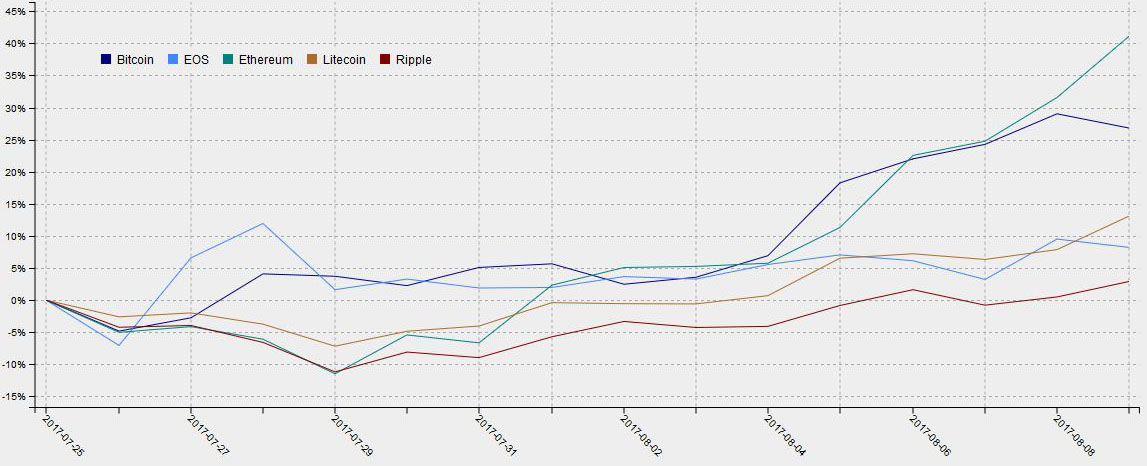
\includegraphics[width=1.0\textwidth]{ROI_short.JPG}
\caption{Retour sur investissement (ROI) de 5 monnaies entre le 25/7/2017 et le 9/8/2017}
\label{fig:roi_short}
\end{center}
\end{figure}

\begin{figure}[ht!]
\begin{center}
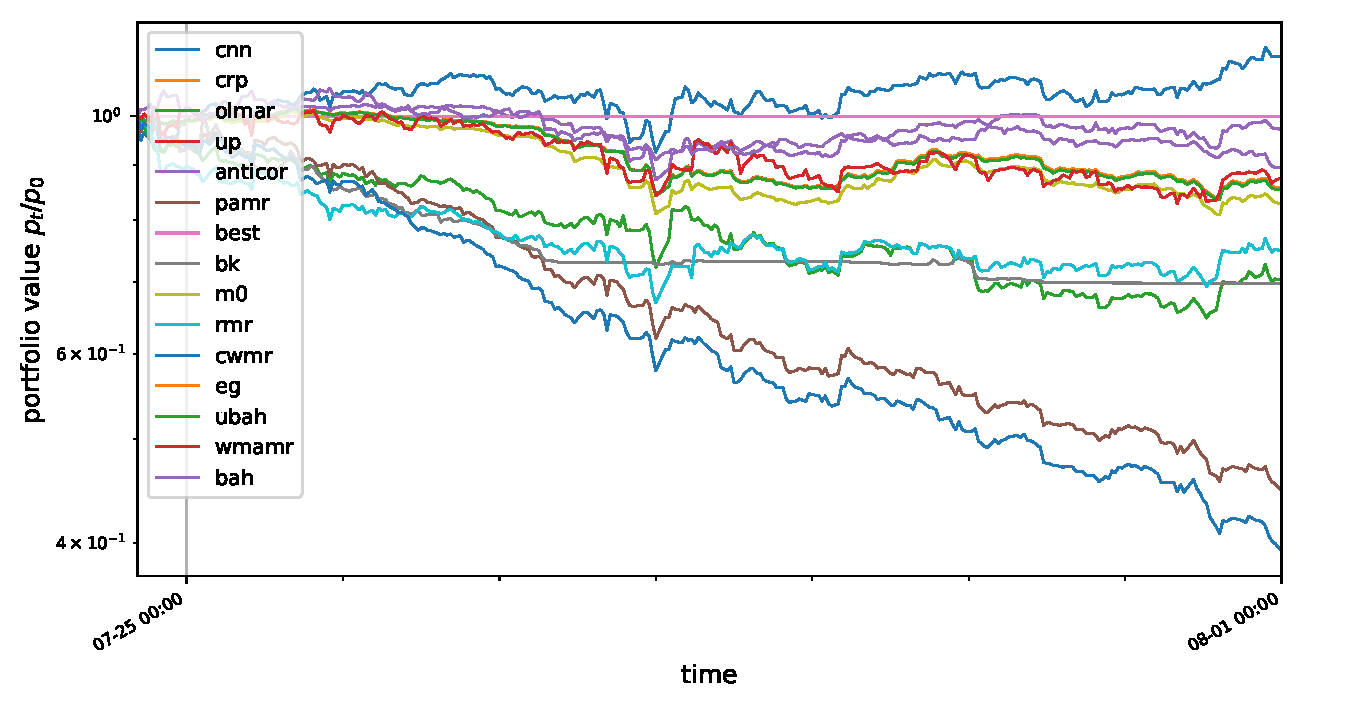
\includegraphics[width=1.0\textwidth]{plot_short.pdf}
\caption{Évolution des portfolios de chaque algorithme (25 juillet au $1^{\text{e}}$ août 2017)}
\label{fig:plot_short}
\end{center}
\end{figure}

\begin{center}
\begin{table}[!ht]
\begin{tabularx}{\textwidth}{YYYYY}
\toprule
\textbf{Algorithme} & \textbf{Croiss. moy.} & \textbf{VF} & \textbf{MDD} & \textbf{RS}\\
\midrule
UBAH    & 0.999503 & 0.857542 & 0.175826 & -0.090797 \\
BAH     & 0.999659 & 0.895841 & 0.156347 & -0.047898 \\
UCRP    & 0.999489 & 0.854162 & 0.177425 & -0.095134 \\
Best    & 1.000000 & \textbf{1.000000} & 0.000000 &  N/A \\
CNN     & 1.000504 & \textbf{1.136845} & 0.154795 &  \textbf{0.040674} \\
Anticor & 0.999930 & 0.972036 & \textbf{0.150485} & -0.009877 \\
OLMAR   & 0.998904 & 0.703084 & 0.342543 & -0.088098 \\
PAMR    & 0.997386 & 0.447489 & 0.551817 & -0.233060 \\
WMAMR   & 0.999633 & 0.876064 & 0.186466 & -0.030030 \\
CWMR    & 0.996959 & 0.393266 & 0.606756 & -0.266809 \\
RMR     & 0.999111 & 0.748939 & 0.327542 & -0.072642 \\
UP      & 0.999502 & 0.857191 & 0.175851 & -0.091108 \\
EG      & 0.999502 & 0.857368 & 0.175913 & -0.091007 \\
BK      & 0.998827 & 0.698287 & 0.298748 & -0.170781 \\
M0      & 0.999393 & 0.828398 & 0.198717 & -0.095927 \\
\bottomrule
\end{tabularx}
\caption{Performance des algorithmes sur une période courte}
\label{tab:perf_short}
\end{table}
\end{center}

Les résultats de cette étude sur court terme, disponibles dans la Table \ref{tab:perf_short}, nous permettent d'apprécier au premier coup d'oeil la suprématie du réseau neuronal convolutif. En plus de dégager le plus grand profit (+13\% de l'investissement initial, en seulement 7 jours), il réussit également à obtenir le ratio de Sharpe le plus faible. Il est suivi par l'algorithme Best, dont la décision a été de conserver l'ensemble de l'investissement en Bitcoin, conservant ainsi la mise initiale et sans risque (le ratio de Sharpe n'est cependant pas calculable dans ce cas là, cf. équation (2)). les autre algorithmes ne réussissent quant à eux pas à dégager de bénéfices sur cette période. On peut toutefois remarquer parmi eux la performance d'Anticor, qui obtient le plus petit maximum drawdown et la plus petite perte.

\subsubsection{Sur du long terme en période "propice"}

On cherche dans cette situation à observer le comportement des algorithmes en période de grande croissance du prix de la majorité des monnaies, afin de mesurer en quelques sortes quels algorithmes profitent le mieux d'une telle situation. On se focalise donc dans ce cas là sur leur capacité à maximiser le gain, le risque étant assez peu présent. Une telle situation décrit par exemple assez bien le climat propice de la fin de l'année 2017, comme le montre la Figure \ref{fig:roi_high}. On choisit donc d'effectuer cette étude sur la période du $1^{\text{e}}$ septembre au $1^{\text{e}}$ décembre 2017. L'évolution des valeurs des portefeuilles dont affichés dans la Figure \ref{fig:plot_high}.

\begin{figure}[ht!]
\begin{center}
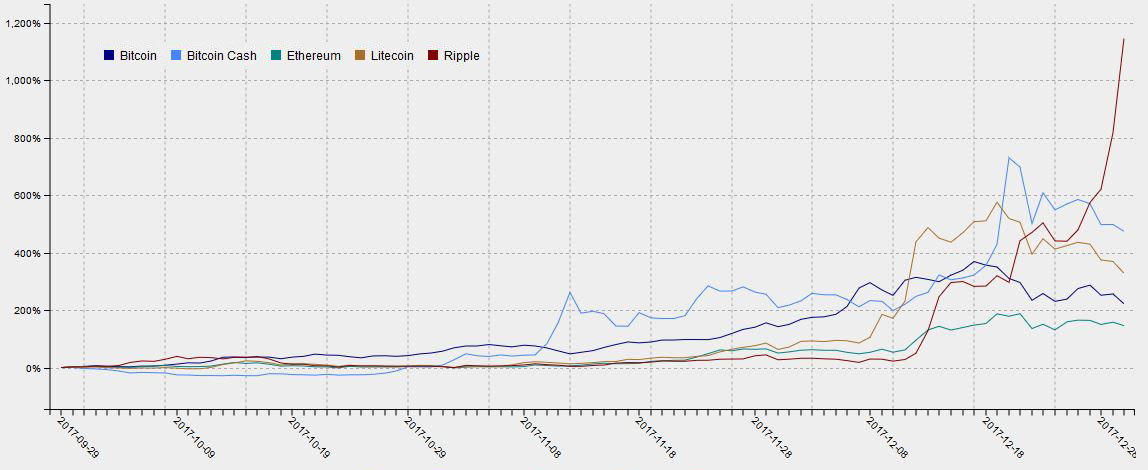
\includegraphics[width=1.0\textwidth]{ROI_high.JPG}
\caption{Retour sur investissement (ROI) de 5 monnaies entre le 29/9/2017 et le 1/1/2018}
\label{fig:roi_high}
\end{center}
\end{figure}

\begin{figure}[ht!]
\begin{center}
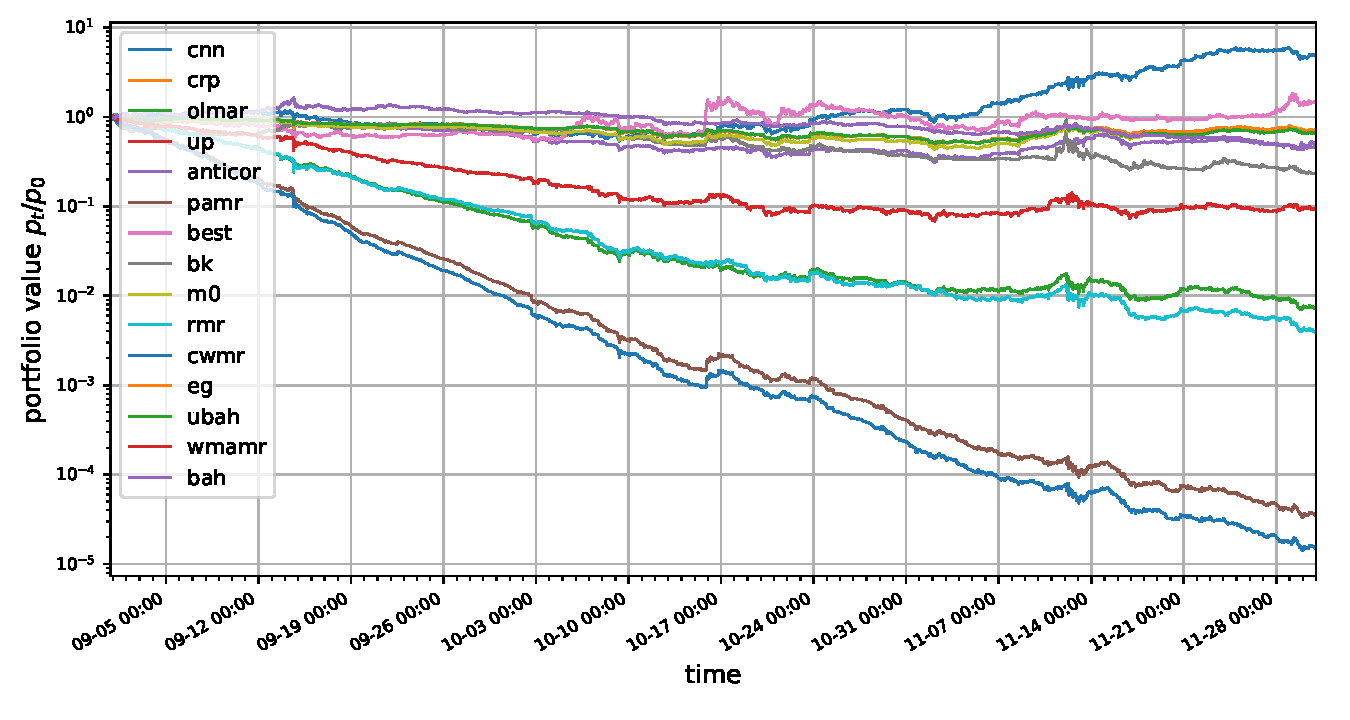
\includegraphics[width=1.0\textwidth]{plot_high.pdf}
\caption{Évolution des portfolios de chaque algorithme ($1^{\text{e}}$ septembre au $1^{\text{e}}$ décembre 2017)}
\label{fig:plot_high}
\end{center}
\end{figure}

\begin{center}
\begin{table}[!ht]
\begin{tabularx}{\textwidth}{YYYYY}
\toprule
\textbf{Algorithme} & \textbf{Croiss. moy.} & \textbf{VF} & \textbf{MDD} & \textbf{RS}\\
\midrule
UBAH    & 0.999940 & 0.713298 & 0.506966 & -0.010091 \\
BAH     & 0.999870 & 0.484452 & 0.737925 & -0.015162 \\
UCRP    & 0.999927 & 0.661413 & \textbf{0.503504} & -0.010777 \\
Best    & 1.000240 & \textbf{1.422701} & 0.585365 &  0.013452 \\
CNN     & 1.000494 & \textbf{4.912568} & 0.542773 &  \textbf{0.031007} \\
Anticor & 0.999873 & 0.466154 & 0.696386 & -0.012878 \\
OLMAR   & 0.998998 & 0.007047 & 0.993178 & -0.059715 \\
PAMR    & 0.997759 & 0.000034 & 0.999967 & -0.138442 \\
WMAMR   & 0.999575 & 0.093635 & 0.934437 & -0.027190 \\
CWMR    & 0.997566 & 0.000015 & 0.999986 & -0.148947 \\
RMR     & 0.998858 & 0.003859 & 0.996357 & -0.068339 \\
UP      & 0.999939 & 0.711239 & 0.506651 & -0.010140 \\
EG      & 0.999939 & 0.711675 & 0.506802 & -0.010129 \\
BK      & 0.999755 & 0.231534 & 0.772612 & -0.017986 \\
M0      & 0.999935 & 0.677607 & 0.577664 & -0.009125 \\
\bottomrule
\end{tabularx}
\caption{Performance des algorithmes sur une période propice}
\label{tab:perf_high}
\end{table}
\end{center}

Les résultats de la Table \ref{tab:perf_high} nous montre malheureusement là encore l'incapacité de la majorité des algorithmes à dégager un bénéfice, même en trois mois de temps et sur une période qui semble le plus propice pour cela. A nouveau, seuls Best et le CNN sont capable d'obtenir un multiplicateur de valeur supérieur à 1, et le CNN s'illustre par sa capacité à multiplier l'investissement initial par 5. Ils sont également les seuls à obtenir un ratio de Sharpe supérieur à 0. L'algorithme Uniform Constant Redistribution Portfolio minimise le maximum drawdown mais perd 34\% de son investissement initial. Certains algorithmes s'illustrent par leur mauvais résultats, comme CWMR et PAMR qui divisent leur capital par plus de 1000, et OLMAR et RMR par près de 100. Ces résultats questionnement largement l'applicabilité des algorithmes de trading "classiques" à des marchés différents de ceux pour lesquels ils ont été pensés, et de leur sur-spécialisation croissante à l'aide de connaissances expertes peut-être toujours trop avancées. Une majorité des algorithmes qui performent le moins bien sont en effet datés des années 2010, tandis que ceux qui s'en sortent le mieux sont les plus anciens (par exemple UP 1991, EG 1998, UCRP 1956, etc.). Nous discuterons plus avant de la sous-jacence d'hypothèses sur le marché dans les modèles des algorithmes lors de leur étude approfondie (partie 3.4).

\subsubsection{Sur du long terme en période "néfaste"}

Les marchés des cryptomonnaies ne demeurant malheureusement pas toujours en pleine expansion, on s'intéresse cette fois à la capacité des algorithmes à limiter les risque, voir la perte, pour les utilisateurs qui utiliseraient notre produit dans une telle période. On étudie donc cette fois les décisions des algorithmes sur la période du $1^{\text{e}}$ janvier au $1^{\text{e}}$ avril 2018, qui correspond à une période de grande chute des prix des monnaies et une faible rentabilité des monnaies, comme illustré par la Figure \ref{fig:roi_low}. L'évolution de la valeur des portfolios de chaque algorithme est disponible dans la Figure \ref{fig:plot_low}.

\begin{figure}[ht!]
\begin{center}
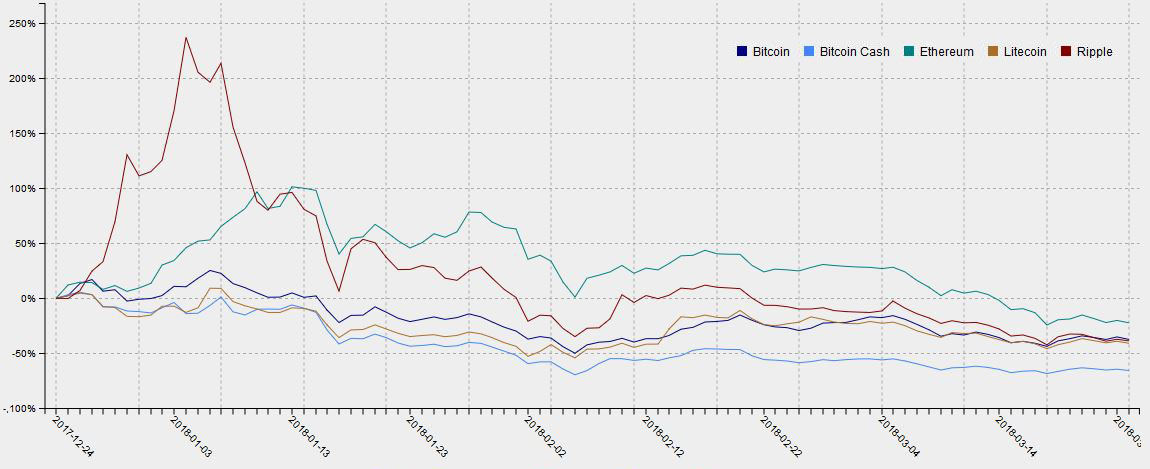
\includegraphics[width=1.0\textwidth]{ROI_low.JPG}
\caption{Retour sur investissement (ROI) de 5 monnaies entre le 24/12/2017 et le 25/3/2018}
\label{fig:roi_low}
\end{center}
\end{figure}

\begin{figure}[ht!]
\begin{center}
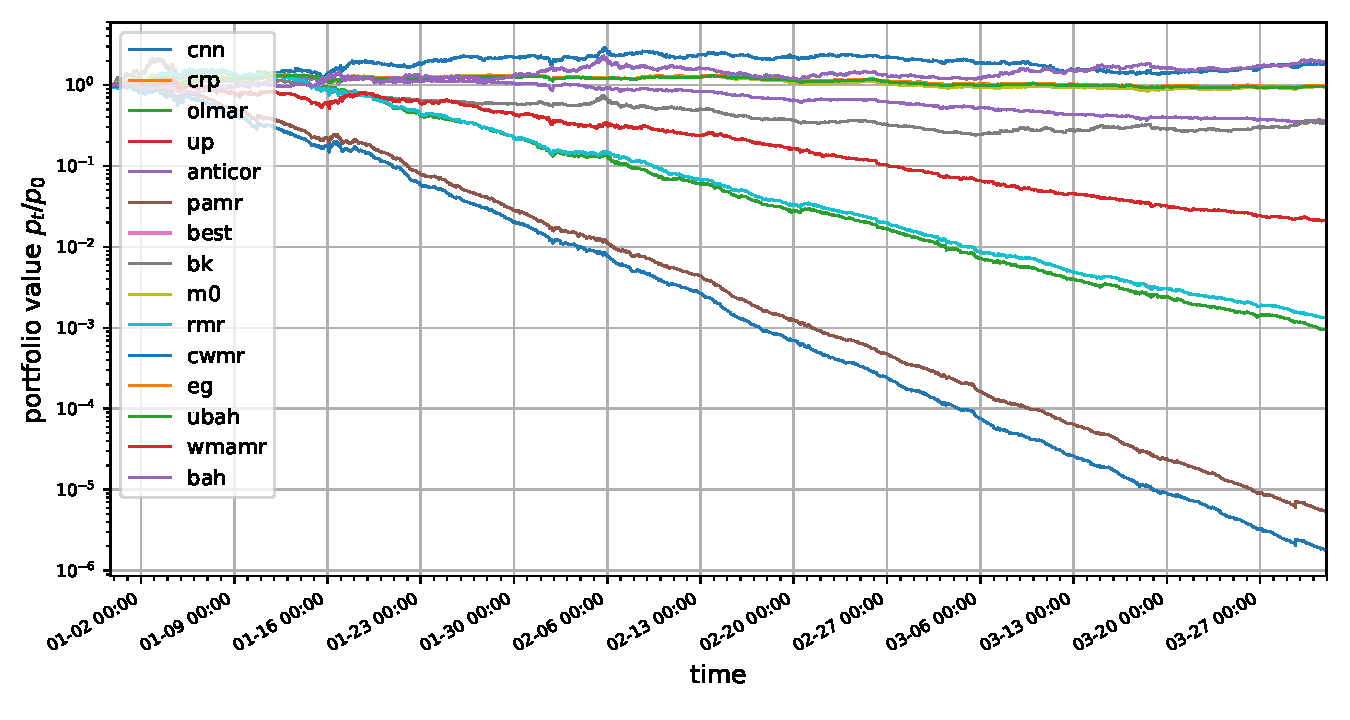
\includegraphics[width=1.0\textwidth]{plot_low.pdf}
\caption{Évolution des portfolios de chaque algorithme ($1^{\text{e}}$ janvier au $1^{\text{e}}$ avril 2018)}
\label{fig:plot_low}
\end{center}
\end{figure}

\begin{center}
\begin{table}[!ht]
\begin{tabularx}{\textwidth}{YYYYY}
\toprule
\textbf{Algorithme} & \textbf{Croiss. moy.} & \textbf{VF} & \textbf{MDD} & \textbf{RS}\\
\midrule
UBAH    & 1.000008 & 0.986813 & 0.309470 &  0.001729 \\
BAH     & 1.000220 & \textbf{1.989104} & 0.488889 &  \textbf{0.019891} \\
UCRP    & 1.000004 & 0.964661 & 0.310212 &  0.000799 \\
Best    & 1.000220 & \textbf{1.989104} & 0.488889 &  \textbf{0.019891} \\
CNN     & 1.000222 & \textbf{1.824969} & 0.536745 &  0.017242 \\
Anticor & 0.999803 & 0.366518 & 0.731929 & -0.023750 \\
OLMAR   & 0.998482 & 0.000969 & 0.999380 & -0.117113 \\
PAMR    & 0.997289 & 0.000005 & 0.999995 & -0.210151 \\
WMAMR   & 0.999186 & 0.021587 & 0.982921 & -0.067846 \\
CWMR    & 0.997031 & 0.000002 & 0.999998 & -0.224027 \\
RMR     & 0.998558 & 0.001357 & 0.999178 & -0.113020 \\
UP      & 1.000008 & 0.985659 & \textbf{0.307534} &  0.001673 \\
EG      & 1.000008 & 0.985941 & 0.308693 &  0.001690 \\
BK      & 0.999814 & 0.346746 & 0.887654 & -0.017139 \\
M0      & 1.000009 & 0.952937 & 0.388243 &  0.001414 \\
\bottomrule
\end{tabularx}
\caption{Performance des algorithmes sur une période néfaste}
\label{tab:perf_low}
\end{table}
\end{center}

Les résultats de l'étude de la Table \ref{tab:perf_low} confortent ceux obtenur précédemment. Le CNN obtient de nouveau de très bons résultats, réussissant à dégager un bénéfice malgré la situation difficile, et doublant presque la valeur de l'investissement. Le portefeuille de Buy and Hold (BAH), qui consiste à tout investir dans le dollar et donc à n'acheter aucune cryptomonnaie, arrive logiquement en seconde position, de même que Best, qui ne peut investir que dans une unique monnaie, qui semble avoir bien détecter l'opportunité de n'acheter que du dollar lui aussi. Ces deux portfolio disposent d'ailleurs du plus fable ratio de Shapre montrant leur sécurité, suivis de peu par le CNN. UP et EG sont de nouveau presque à l'équilibre mais accusent une légère perte mais disposent de très bonnes valeur de maximum drawdown.

\subsection{Étude des algorithmes retenus}

Les études de la section précédentes nous ont montrés qu'un petit groupe d'algorithmes présente souvent les meilleurs résultat. Ce sont ces six algorithmes que l'on décide de conserver, d'implémenter dans notre produit et de proposer aux utilisateurs. Il s'agit de Uniform Constant Redistribution Portfolio (UCRP), Best Stock (Best), le réseau neuronal convolutif (CNN), Exponential Gradient (EG), Universal Portfolio (UP) et Anticor. Dans la suite, nous étudions en détail les principes sur lesquels ils reposent.

\subsubsection{Uniform Constant Redistribution Portfolio}

Longuement étudié par \citet{Cover1991}, cette stratégie illustre le succès que la simplicité peut encore avoir dans des situations avec si peu de connaissances expertes certaines. Considéré aujourd'hui comme un algorithme de référence, seulement utilisé pour comparaison avec des algorithmes plus poussés, cet algorithme est un cas particuliers des algorithmes de stratégie "Constant Redistribution Portfolio". Celle-ci repose sur l'idée simple de balancer à chaque période $t$ le portfolio vers un portfolio fixe $\omega$, soit en d'autre termes : $\forall t \in [0, T],\ \omega_t^{\text{\tiny CRP}} = \omega$. La stratégie UCRP est celle pour laquelle le portfolio fixe est répartie équitablement entre chaque monnaie, c'est à dire :
\begin{equation}
    \omega_t^{\text{\tiny UCRP}} = \left(\frac{1}{m}, \frac{1}{m}, ..., \frac{1}{m} \right) \quad \forall t \in [0, T], \text{ avec un portfolio de $m$ monnaies} 
\end{equation}

Elle est cependant à différencier de la stratégie Buy and Hold et de son pendant Uniform Buy and Hold en cela que la stratégie BAH ne touche pas à la répartition des monnaies après avoir fixer le portefeuille au temps $t=0$. Dans UCRP, si la valeur de l'une des monnaies change, par exemple augmente fortement, la valeur du portefeuille est recalculée puis la part allouée à celle monnaie sera réduite, pour conserver une distribution de valeur égale entre toutes les monnaies.

\subsubsection{Best Stock}

Développé également dans \cite{Cover1991}, l'algorithme Best est également un algorithme utilisé le plus souvent en référence. Dans l'étude empirique réalisé précédemment, il surpasse pourtant toutes les autres stratégies, à l'exception de celle du NN. Best est un cas particulier d'algorithme Buy and Hold, stratégie qui fonctionne comme on l'a vu précédemment avec un portfolio fixé à $t=0$ puis non modifié. Sa valeur cumulative finale est donc :
\begin{equation}
    VF = \omega_0^{\text{\tiny BAH}} \cdot \left( \bigodot_{t=0}^{T} y_t \right)
\end{equation}
avec $\bigodot$ l'opérateur de produit terme à terme, $\cdot$ le produit scalaire, et $y_t$ le vecteur de prix des monnaies à la période $t$.

Partant de cette simple formule, l'idée de l'algorithme Best est de trouver le portefeuille fixe qui aurait maximisé le gain sur une période antérieure à la date de début du trading on-line, idéalement finissant à la date où celui-ci commence. Le vecteur fixe de poids choisi par cet algorithme est donc :
\begin{equation}
    \omega_0^{\text{\tiny Best}} = \argmax_{\omega \in \Omega_m} \left( \omega \cdot \left(\bigodot_{t=0}^{T} y_t \right)\right)
\end{equation}

\subsubsection{Exponential Gradient}

L'algorithme EG, développé par \citet{Helmbold1998}, appartient à la catégorie des approches "Follow-the-Winner", c'est à dire une approche dont l'hypothèse sous-jacente est qu'un actif ayant été performant à une période $t$ devraient également l'être au temps $t+1$. Contrairement aux algorithmes précédents, l'approche de EG est on-line, c'est à dire que la décision du prochain portfolio se fait en fonction des résultats du temps présent. Exponential Gradient est formulé comme le problème d'optimisation suivant :
\begin{equation}
    \omega_{t+1}^{\text{\tiny EG}} = \argmax_{\omega \in \Omega_m} \left( \eta \log \left(\omega \cdot y_t - R(\omega, \omega_t) \right) \right)
\end{equation}
où $\eta > 0$ est le coefficient d'apprentissage et $R(\omega, \omega_t)$ dénote le terme de régularisation. On peut globalement interpréter cette équation comme une recherche du portfolio avec la meilleure performance à la période précédente mais avec une volonté de garder le portfolio suivant proche du précédent. Le terme de régularisation employé est l'entropie relative : 
\begin{equation}
    R(\omega, \omega_t) = \sum_{i=1}^{m} \omega(i) \log \frac{\omega(i)}{\omega_{b}(i)}
\end{equation}

Les auteurs montrent par la suite que ce problème peut être reformulé de la sorte, en utilisant une expansion de Taylor du premier ordre sur $\omega_t$:
\begin{equation}
    \omega_{t+1}^{\text{\tiny EG}}(i) = \frac{1}{k} \ \omega_{t}(i) \ \exp \left(\eta \frac{y_{t}(i)}{\omega_{t} \cdot y_t} \right) \quad \forall i \in [1, ..., m]
\end{equation}
où $\omega(i)$ désigne le $i^{\text{ème}}$ terme de $\omega$ (soit le poids associé à la monnaie $i$), et $k$ est le terme de normalisation qui assure que les poids du vecteurs somment à 1.

\subsubsection{Universal Portfolio}

Imaginé également dans \cite{Cover1991}, la stratégie UP est également de type "Follow-the-Winner". Son idée est de calculer les performances de tous les portfolios valide au cours des périodes écoulées, puis d'en effectuer un mixage pondéré par ces performances de gains. Formellement, la procédure est la suivante :
\begin{equation}
    \omega_{t+1}^{\text{\tiny UP}} = \int_{\Omega_m} \omega S_t(\omega) \ d\omega \bigg/ \int_{\Omega} S_t(\omega) \ d\omega
\end{equation}
où l'intégration se fait donc sur $\Omega_m$, l'ensemble des portfolios valides, et $S_t(\omega)$ est défini par :
\begin{equation}
    S_t(\omega) = \prod_{k=1}^{t} \omega \cdot y_t
\end{equation}

L'apparente difficulté dans la formulation et la compréhension de cet algorithme se retrouve dans sa complexité temporelle, puisque cette dernière est de $O(n^m)$ avec $n$ le nombre de périodes et $m$ le nombre de monnaies. Il existe une large littérature qui s'intéresse aux possibilités de son amélioration, notamment pour le calcul des poids $S_t$.

\subsubsection{Anticor}

Anticor, pour anti-corrélation, suit pour sa part une approche "Follow-the-Loser", basée sur l'intuition qu'un actif ayant eu de mauvais résultats à une période est plus susceptible d'en avoir des bons à la période suivante. Contrairement par exemple à UP, qui ne fait aucune hypothèse de distributions, la stratégie d'Anticor repose sur l'hypothèse que le marché suit le principe de mean reversion, selon lequel le prix d'un actifs tendra à évoluer vers son prix moyen. Elle cherche à l'exploiter en pariant sur la consistance de corrélations croisées retardées, et d'auto-corrélation négative récentes.

Elle s'intéresse donc à deux fenêtres temporelles pour les prix : $X_1 = \log \left(y_{t-2\alpha+1}^{t-\alpha} \right)$ et $X_2 = \log \left(y_{t-\alpha+1}^{t}\right)$, deux matrices extraites de $y_t$ pour une fenêtre de temps donnée $\alpha$ et passées au log. Elle utilise ensuite aux matrices de corrélation croisées entre $X_1$ et $X_2$ : 
\begin{equation}
    M_{cov}(i, j) = \frac{1}{\alpha - 1}(X_{1}(i) - \mu_1(i))^{T}(X_2(j) - \mu_2(j))
\end{equation}
et
\begin{equation}
    M_{cor}(i, j) =
        \begin{cases}
            \frac{M_{cor}(i,j)}{\sigma_1(i)\sigma_2(j)} & \text{si } \sigma_1(i), \sigma_2(j) \ne 0 \\
            0                                           & \text{sinon}
        \end{cases}
\end{equation}
où $\mu_k = (\mu_k(1), ..., \mu_k(m))$ est le vecteur des moyennes des colonnes de $X_k$, et de même $\sigma_k$ celui des écarts-types.

Finalement, la décision de redistribution des poids entre les monnaies $i$ et $j$ ne se fait que si l'on détecte une corrélation entre ces deux monnaies, et que la première monnaie se déplace "plus rapidement" que la seconde, i.i. ssi $M_{cor}(i,j) > 0$ et $\sigma_2(i) > \sigma_2(j)$. Dans ce cas, la quantité de monnaie à déplacer de $i$ à $j$, disons $d_{i\rightarrow j}$ est proportionnelle à cette corrélation ainsi qu'à l'auto corrélation de chaque monnaie. On peut écrire ce processus sous forme algorithmique :
\begin{equation}
    \forall i, j \in [1, ..., m], d_{i\rightarrow j} =
        \begin{cases}
            M_{cor}(i,j) + A(i) + A(j) & \text{si } M_{cor}(i,j) > 0 \text{ et } \sigma_2(i) > \sigma_2(j) \\
            0                          & \text{sinon}
        \end{cases}
\end{equation}
avec
\begin{equation}
    A(k) = 
    \begin{cases}
        |M_{cor}(k,k)| & \text{si } M_{cor}(k,k) < 0 \\
        0              & \text{sinon}
    \end{cases}
\end{equation}

La ré-allocation de poids est finalement :
\begin{equation}
    \omega_{t+1}^{\text{\tiny Anticor}}(i) = \omega_{t}(i) + \sum_{i \ne j} \left(t_{j\rightarrow i} - t_{i\rightarrow j} \right)
\end{equation}
avec $t_{j\rightarrow i}$ le transfert de $i$ à $j$ défini par
\begin{equation}
    t_{j\rightarrow i} = \frac{\omega_{t}(i) \cdot d_{i\rightarrow j}}{\sum_{j} d_{i\rightarrow j}}
\end{equation}

\subsubsection{Le réseau neuronal convolutif}

Comme expliqué plus tôt, cet algorithme a été imaginé et présenté par dans un article par \citet{Jiang2017}. Le principe de cet algorithme est de se débarrasser de toute modélisation ou hypothèses sur l'évolution du marché, contrairement par exemple aux approches Follow-the-Winner ou Follow-the-Loser. En procédant ainsi, nos expériences ont montré qu'on obtenait des résultats bien supérieurs, mais on sacrifie dans un même temps toute capacité à expliquer la logique derrière la décision prise par l'algorithme. La domination du CNN semble ainsi montrer que les logiques de fluctuation des marchés financiers (et de celui des cryptomonnaies en particulier) sont loin d'être comprises, et que les connaissances expertes qui ont été conçues et testées sur des marchés boursiers classiques (voir les résultats de \cite{Li2014}) ne donnent pas des résultats aussi bons sur les marchés de nouveaux types d'actifs comme les cryptomonnaies.

Le principe général de l'algorithme est de suivre un apprentissage par renforcement, avec utilisation d'un politique déterministe. L'environnement est défini comme le marché financier des cryptomonnaies, et l'état de l'agent (sa connaissance de l'environnement) comme les prix actuels et passés des monnaies, considérés traditionnellement par les analystes financiers \cite{Lo2000}. L'état d'un agent à un temps $t$ est donc simplement défini par le portefeuille qu'il hérite du temps précédent et d'un tenseur de prix $X_t$ : $s_t = (X_t, \omega_{t-1})$. Il dispose également d'une fonction de reward, directement induite par la valeur finale du portfolio $p_T$:
\begin{equation}
    p_T = p_0 \prod_{t=1}^{T+1} \mu_t \ y_t \cdot \omega_{t-1}
\label{eq:valeur_finale}
\end{equation}
où $p_0$ désigne l'investissement initial, $y_t$ le vecteur de prix des monnaies au temps $t$, $\omega_t$ le vecteur de poids du portfolio, et $\mu_t$ un facteur de réduction, par excellence $1 - c$ où $c$ désigne le taux de commission. La fonction de reward n'est autre que la moyenne logarithmique de cette valeur :
\begin{equation}
    R = \frac{1}{T} \sum_{t=1}^{T+1} \ln(\mu_t \ y_t \cdot \omega_{t-1})
\end{equation}
Enfin, la politique (qui n'est autre qu'une fonction de projection de l'espace d'état vers celui des actions, i.e. $\pi_{\theta} : S \mapsto A$, est obtenue grâce à un algorithme de montée de gradient, où la  métrique de performance n'est autre que le reward associé au paramètres $\theta$ : $R(s_1, \pi_{\theta} (s_1), ...s_T, \pi_{\theta} (s_T), s_{T+1})$. Il est intéressant de noter que cet agent va donc simplement chercher à maximiser son profit sans s'intéresser au risque encouru, mais réussit tout de même à minimiser ce dernier comme nous l'avons vu au cours des tests empiriques.

La structure adoptée pour l'implémentation de cet agent est celle d'un réseau neuronal convolutif (CNN) appliqué à la prédiction de portefeuille comme pourrait le faire un CNN classique appliqué à la reconnaissance d'image. Il prend en entrée une matrice de taille $3 \times m \times n$, où 3 correspond aux trois features "closing" (prix d'échange), "highest" (prix le plus haut) et "low" (prix le plus bas), $m$ au nombre de monnaies choisies (hors monnaie de réserve) et $n$ la fenêtre de temps i.e. un nombre de périodes précédentes. L'algorithme prend également en entrée le portfolio de la période précédente, pour permettre à l'algorithme de minimiser les coûts de transaction.

La structure du réseau est basée sur une dichotomie avec celle des CNN utilisés pour la détection d'image, où les 3 valeurs RGB sont remplacées par les 3 valeurs des features. L'astuce de la structure employée est que les $m$ lignes correspondant aux $m$ monnaies sont traitées sur des réseaux identiques mais indépendants (EIIE, Ensemble of Identical Independent Evaluators), et ne s'interconnectent qu'à la fin en un vote (scoring) utilisant une fonction softmax pour garantir la non-négativité des portfolio prédits et la sommation à 1. La Figure \ref{fig:structure}, tirée de l'article cité plus tôt, résume cette organisation : on observe une décomposition 4 convolutions, où les lignes ne se mélangent jamais. Le portfolio de l'étape précédente entre eu jeu à la 3e étape, et la monnaie de réserve uniquement à la 4e, lors de l'agrégation des résultats des IIE. \citet{Jiang2017} ont implémenté cette structure de convolutions sous Tensorflow, structure que nous avons repris dans notre projet.

\begin{figure}[ht!]
\begin{center}
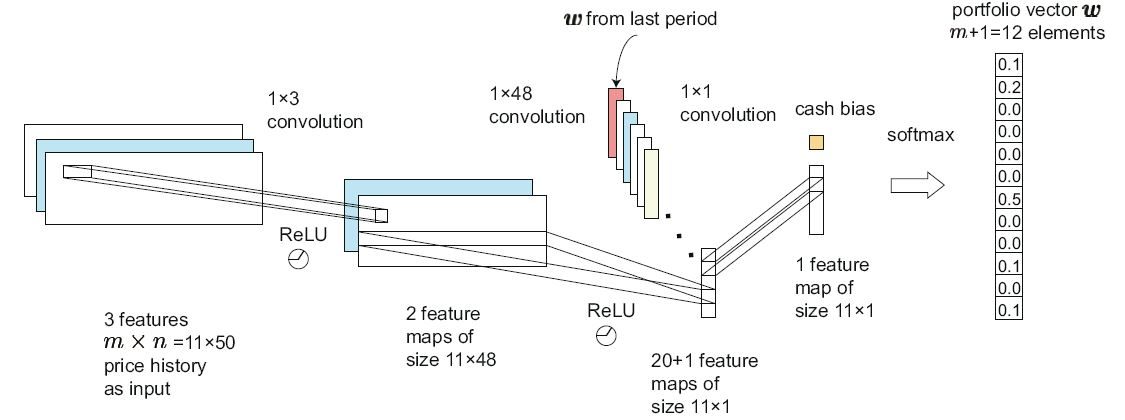
\includegraphics[width=1.0\textwidth]{structure.JPG}
\caption{Structure du réseau neuronal convolutif (CNN)}
\label{fig:structure}
\end{center}
\end{figure}

Le CNN est sensible à plusieurs paramètres, qu'il est nécessaire de fixer pour une utilisation future au sein du logiciel. Il ne fait en effet pas beaucoup de sens que ce soit à l'utilisateur lambda de paramétré et entraîner son réseau de neurones. On retiendra notamment pour $n$, le nombre de périodes à considérer dans notre matrice $X_t$, la valeur  $n = 50$, une fenêtre assez large pour fournir des données fortement corrélées (très proches dans le temps) et peu corrélées (plus anciennes) à l'algorithme, et qui correspond à la valeur conseillée par les auteurs après étude personnelle. Le nombre de monnaies $m$ doit rester customisable par l'utilisateur, mais ce point sera discuté plus en long dans la partie 4.4.1. Enfin, le dernier paramètre important est la fréquence des données passées en entraînement. Dans les tests réalisés plus tôt, nous avions arbitrairement fixé cette période à 30 minutes, mais l'API de Poloniex nous offre de plus nombreuses possibilités. La Table \ref{tab:cnn_compar} ne semble montrer aucune réelle supériorité entre les CNN entraînés avec les fréquences 5 minutes, 30 minutes et 4h, sur la période du $1^{\text{e}}$ septembre au $1^{\text{e}}$ décembre 2017. Nous choisirons donc de fixer cette fréquences à 30 minutes, fréquence également utilisée par \citet{Jiang2017}, parce qu'elle semble correspondre à la fréquence maximale qu'un utilisateur puisse faire de notre outil sans avoir plutôt besoin d'un outil de trading haute fréquence, et elle permet également de garantir que l'ensemble des ordres d'achat ou de vente pourront être passés et exécutés avant une prochaine optimisation, notamment sur des marchés avec une plus faible liquidité.

\begin{center}
\begin{table}[!ht]
\begin{tabularx}{\textwidth}{YYYY}
\toprule
\textbf{Algorithme} & \textbf{VF} & \textbf{MDD} & \textbf{RS}\\
\midrule
CNN (freq. 5min)    & 0.964661 & 0.310212 &  0.000799 \\
CNN (freq. 30min)   & 1.989104 & 0.488889 &  0.019891 \\
CNN (freq. 4h)      & 1.824969 & 0.536745 &  0.017242 \\
\bottomrule
\end{tabularx}
\caption{Performances de 3 CNN entraînés avec des fréquences différentes}
\label{tab:cnn_compar}
\end{table}
\end{center}

\newpage
\section{Développement logiciel}

Dans cette partie, nous aborderons les étapes et les choix effectués pour l'intégration des algorithmes précédemment choisis vers la création d'une interface d'aide à la décision en ligne pour un utilisateur sans connaissance du sujet. Nous décrirons succinctement l'organisation des tâches qui a été suivie, puis rentrerons dans le détail des fonctionnalités proposées et de leur disposition au sein de l'interface, avant de discuter des choix techniques qu'il a été nécessaire de réaliser.

\subsection{Organisation des tâches}

\subsubsection{Étapes de développement}

- les différentes étapes de développement (parler de la conception (= détournement) des algorithmes, de la conception de Django, des améliorations itératives de l'interface, etc)

\subsubsection{Calendrier}


\subsection{Description du produit}

\subsubsection{Fonctionnalités}

Les fonctionnalités disponibles : refaire une description des différentes pages, de ce qu'il y a : un optimiseur, une interface de suivi de la valeur du portfolio, des graphes (?), etc

\subsubsection{Interface graphique utilisateur}


\subsection{Choix techniques}

Plusieurs choix techniques ont du être réalisés pour l'implémentation de la plate-forme d'optimisation. Nous détaillons ci-dessous les principales, et les motivations qui nous ont poussés à les adopter.

\subsubsection{Connexion et stockage des données des utilisateurs}

L'un des objectifs de notre produit est de pouvoir fournir aux utilisateurs un suivi de leurs portfolios, en plus de la possibilité de les optimiser. Il est donc nécessaire que ceux-ci disposent d'une possibilité de s'identifier, et donc de posséder espace personnel avec connexion sécurisée. Nous avons donc fait le choix d'imposer la création d'un login et d'un mot de passe pour la première utilisation du site, et une nécessité de se connecter pour y accéder par la suite. Les données relatives à ces identifiant sont stockés dans une base de donnée intégrée à Django.

Les informations relatives aux portfolios des utilisateurs sont quant à elles stockées (???).

\subsubsection{Récupération des données relatives aux cryptomonnaies}

L'optimisation des portfolios, tout comme l'affichage des cours des monnaies ou le suivi de l'évolution de la valeur des portfolio, nécessite l'accès à des données en temps réel des prix de ces monnaies. Nous avons pour cela fait le chois d'utiliser l'interface de programmation (API) de la plate-forme d'échange Poloniex, l'une des plus large plate-forme à l'heure actuelle. Celle-ci est en effet facile d'utilisation grâce à des requêtes simples, et propose un temps de réponse très court quel que soit la taille des données demandées. C'est également pour cette raison que nous avons choisi, pour l'ensemble des instruments de notre produit, de ne pas utiliser de base de données pour stocker les informations nécessaires mais d'interroger à chaque fois l'API. Nous avons en effet constaté, après avoir travaillé avec le code source de l'article de \citet{Jiang2017} qui utilisait pour sa part une base de données, que deux inconvénients se présentaient. Tout d'abord celui de l'espace, puisque la taille de la base de données croît rapidement avec l'ajout de points de données, jusqu'à peser plus d'un demi Go pour les données d'une dizaine de mois. La seconde, qui lui est liée, est celle du temps : si une économie de temps pouvaient être réalisée grâce à la constitution de la base puis aux requêtes SQL lorsque les données devaient être lues de nombreuses fois, elle devient inutile lorsqu'on ne souhaite y accéder qu'une fois périodiquement, comme dans le cas de l'optimisation du portefeuille.

\subsubsection{Fréquence et données d'entraînement du CNN}

L'une des décisions associée à l'utilisation du CNN est celle de la fréquence de ré-entraînement de celui-ci, problématique fortement liée à celle de la quantité de données passées en input pour cet entraînement. Ces deux paramètres auraient sûrement mérité une étude de choix empiriques plus approfondie, cependant nous ne pourrons la réaliser ici par manque de temps.

Pour le choix de la quantité de données, nous basons notre raisonnement sur le théorème d'approximation universelle \cite{Hornik1991}, selon laquelle un réseau neuronal à propagation avant composé d'un nombre fini de neurones (perceptrons) et dotés d'une fonction d'activation continue, croissante, non-constante et bornée peut approximer n'importe quelle fonction continue sur un sous-ensemble de $\mathbb{R}^n$. Les hypothèses sont bien vérifiées dans notre CNN, puisque celui-ci utilise une fonction Rectified Linear Unit (RELU, définie par $g(x) = \max(0, x)$) dans les convolutions du EIIE, puis une fonction softmax pour les combiner. Il est de plus évident qu'il existe une infinité de fonctions $f \colon y_t \mapsto \omega_t$ continues et définies de $\mathbb{R}^m$ vers $\Omega_m \subset \mathbb{R}^m$, dont on chercherai à maximiser l'argmax de l'équation \eqref{eq:valeur_finale}. A partir de ce théorème, on peut donc écarter un questionnement sur le fait de donner "trop" de données en entraînement à l'algorithme, et notamment des données "trop anciennes". Le théorème d'approximation universelle et cette équation nous indiquent en effet que le CNN cherchera la fonction qui maximise la valeur amortie, et donc celui qui se comporte mieux en moyenne, et donc dans toutes les situations possibles. s'il est légitime de penser que les mouvements de marché actuels sont plus ressemblant aux mouvements du passé proche de d'un passé plus ancien, ce raisonnement nous pousse à penser qu'il est moins risqué de fournir de nombreux motifs en entraînement, fussent-ils obsolètes. On choisit donc de fournir à l'algorithme les matrices de valeur des monnaies $X_t$ sur deux ans précédant la date actuelle.

A partir de cette décision, il nous semble légitime de penser que l'ajout de quelques dizaines de périodes à la matrice $X_t$, voir même de quelques centaines, ne changera pas fondamentalement le résultat (la matrice $X_t$ contiendra en effet $2 \times 365 \times 24 \times 2 = 35 040$ période, une dizaine semblent marginales). Il est cependant nécessaire d'être conscient que cette hypothèse pourrait s'avérer fallacieuse, puisque l'on ne peut connaître l'importance relative donnée à chaque période par le CNN en fonction de son ancienneté. A partir de celle-ci cependant, nous avons décidé que le ré-entraînement s'effectuerait tous les 7 jours (soit un changement de $336$ périodes).

\subsection{Limitations du produit final}

Par manque de temps ou face à des limitations techniques, certaines caractéristiques initialement prévues dans le projet ont dues être revues à la baisse ou supprimées. Nous les détaillons dans la suite ainsi que les choix techniques que nous avons réaliser pour les contourner.

\subsubsection{Nombre de portefeuilles possibles}

L'un des problèmes majeurs liés à l'utilisation du réseau neuronal convolutif est lié à sa nécessité d'un entraînement en fonction de chaque situation. Nous avons discuté plus tôt des modalités liées à la fréquence des points de données (on a retenu 30 minutes entre chaque), celles liées à l'actualisation du réseau avec l'arrivée de nouvelles données (et donc le choix de la fréquence à laquelle le ré-entraîner), mais il reste à discuter la principale difficulté liée au choix des monnaies. En effet, si $M$ est le nombre de monnaies disponibles, alors le nombre de portefeuilles possibles est $2^M - 1$. Si l'on se restreint à la plate-forme Poloniex seule, qui propose un peu plus de 80 monnaies, cela représente plus de $10^{24}$ portefeuilles que l'utilisateur peut demander à notre produit d'optimiser, et donc tout autant de réseaux entraînés à avoir sous la main ! Face à cette difficulté, un premier choix a été de limiter le nombre de monnaies disponibles au choix sur notre plate-forme à $12$, à savoir les $11$ monnaies principales en terme de capitalisation de marché en plus du Bitcoin (et du dollar) : Ethereum, Ripple, Bitcoin Cash, EOS, Litecoin, Cardano, Stellar, IOTA, TRON, NEO, Monero et Dash. En plus de présenter une facilité pour le CNN, cette solution permet d'assurer que la liquidité des monnaies sélectionnées sera toujours suffisante pour que les ordres de l'utilisateur (achat ou vente) puissent être exécutés.

Mais cette solution nous rapporte tout de même à plus de $4000$ configurations en considérant que Bitcoin et dollar doivent nécessairement y apparaître, et reste impossible à envisager puisque l'entraînement d'un CNN nécessite dans le meilleur cas 2 à 3h, et nécessite entre 2 et 6 Mo d'espace de stockage. La solution que nous avons décidé d'adopter dans le rendu actuel s'appuie donc sur un constat que nous avons fait sur le portefeuille $\omega^{\text{\tiny CNN}}$ conseillé par le CNN : celui-ci est bien souvent composé d'une unique monnaie, parfois de 2 à 3, mais rarement de plus. En s'appuyant sur cette caractéristiques, on procède de la sorte : quelles que soit les monnaies sélectionnées par l'utilisateur, la plate-forme interroge le CNN sur l'affectation optimale avec les 14 monnaies. Si les 1 à 3 monnaies conseillées par lui sont présente dans le portefeuille souhaité l'utilisateur sont présentes, on output $\omega^{\text{\tiny CNN}}$ tel quel. Si certaines ne le sont pas, on supprime la ou les monnaies absentes puis on normalise sur celles présentes. Si aucune n'est présente, on indique à l'utilisateur que l'algorithme ne peut trouver de solution avec sa sélection et lui en conseille une autre basée sur $\omega^{\text{\tiny CNN}}$.

\subsubsection{Automatisation et modularité de l'implémentation}

Comme nous l'avons vu dans la partie 4.3.3, il est nécessaire de ré-entraîner périodiquement notre CNN sous Tensorflow, une fois par semaine par notre chois. Nous souhaitions dans un premier temps automatiser ce processus, de manière à ce que l'entraînement se déclenche sur le serveur à heure fixée. Cependant, cette fonctionnalité n'a pas pu être implémentée par manque de temps. Elle nécessiterait en effet la rédactions de quelques scripts pour le lancement de l'entraînement du réseau et la suppression des plus anciens, sans interrompre la continuité du service. Pour l'heure, nous nous contentons d'entraîner le CNN en local puis de transférer les fichiers du réseau Tensorflow en ligne. Nous avons en effet volontairement choisi de nous focaliser sur les fonctionnalités axées utilisateurs, comme l'amélioration du design ou la possibilité d'enregistrer des portfolios lorsque le temps nous manquait.

Le problème duquel découle ce problème est le manque de modularité de notre code. En effet, si celui-ci fonctionne parfaitement pour l'optimisation à un temps donné, il est assez peu adaptable à d'autre cadres. On peut par exemple penser aux tests sur des données passées, pour lesquels nous avons dû passer par code de \cite{Jiang2017}, ou encore à la mise en production à large échelle avec une automatisation performante de l'enregistrement des données des monnaies ou de d'entraînement du CNN.

\newpage
\section*{Conclusion et ouverture}
\label{sec:conclu}
\addcontentsline{toc}{section}{\nameref{sec:conclu}}

L'implémentation actuelle du produit répond à la problématique initiale : permettre à des utilisateurs sans connaissances sur les cryptomonnaies ou l'optimisation de portefeuille de disposer d'un outil de conseil pour la prise de décision sur l'investissement dans les monnaies virtuelles. Le développement de cette plate-forme a également été l'occasion de s'intéresser à l'applicabilité des algorithmes de trading à des marchés d'un nouveau type, celui des cryptomonnaies, et de constater à quel point les stratégies d'optimisation de portefeuilles classiques sont peu performantes sur ces derniers, alors que les taux de croissances affichés sont très largement supérieurs aux actifs boursiers sur lesquels ils sont traditionnellement appliqués. Ce étude montre donc qu'il est nécessaire de repenser les modèles et les hypothèses sur le marché sur lesquels ces stratégies reposent, mais également que l'étude des marchés des cryptomonnaies est encore un domaine trop peu exploré par les chercheurs en finance alors qu'il présente des caractéristiques tout à fait uniques. Le succès du réseau neuronal convolutif semble montrer qu'il existe bien des patterns reconnaissables pour anticiper les mouvements de valeurs, cependant les connaissances expertes actuelles ne peuvent les déceler.

Ce projet appelle bien entendu de nombreuses extensions et améliorations. Il serait par exemple nécessaire d'améliorer le temps de calcul des algorithmes de recommandation de portfolios, celui-ci atteignant souvent plus d'une dizaine de seconde, durée supérieure à ce qu'un utilisateur attend aujourd'hui d'un site internet. Plusieurs autres fonctionnalités pourraient être intégrées à la plateforme, comme par exemple des suivis d'évolution de valeurs et d'échange plus précis, une plus grande customisation des valeurs à suivre, ou encore la possibilité de suivi sur du long terme de l'évolution d'un portefeuille. L'extension par excellence serait celle de la possibilité de passer des ordre directement depuis la plate-forme : l'utilisateur obtiendrait le portefeuille conseillé par l'algorithme de son choix puis ordonnerait à la plate-forme d'effectuer le changement de portefeuille sur la plate-forme d'échange sur laquelle celui-ci est constitué. Une autre avancée pourrait être de proposer les données d'un plus grand nombre de plate-forme d'échange afin d'augmenter le nombre de monnaies disponibles. Le développement ultime pourrait enfin être de permettre à l'utilisateur de donner le contrôle quasi-total de son portefeuille à notre outil, et que celui-ci gère sa ré-optimisation à fréquence élevée pour permettre une maximisation des profits sans contraindre l'utilisateur à revenir en permanence sur la plate-forme.

\newpage
\printbibliography[heading=bibintoc]

\end{document}
